\subsubsection{Dimensionierung}
Die Dimensionierung erfolgte für eine Verstärkung von $V = 5$ mit den
Widerständen $R_1 = R_3 = 10 \, \si{\kilo\ohm}$. $R_2$ und $R_4$ bestimmen sich
durch
\[R_2 = R_4 = 5 \cdot R_{1/3} = 50 \, \si{\kilo\ohm}\]

\subsubsection{Gleichtaktverstärkung}
Zur Ermittlung der Gleichtaktverstärkung wurden die beiden Eingangsspannungen
gleich gewählt (verbunden) und der Effektivwert der Ausgangsspannung bei den
Frequenzen $f = 1\, \si{\kilo\hertz}$ und $f = 10 \, \si{\kilo\hertz}$ gemessen.
(Eingangsamplitude: $8 \, \si{\milli\volt}_{\mathrm{pp}} = 2.828 \, \si{\milli\volt}_{\mathrm{RMS}}$)

Da die Ausgangsspannung verrauscht war, musste am Oszilloskop zuerst über
\inlinecode{AQUIRE...Mittelwert} das Rauschen durch Mittelung
entfernt werden (Abb. \ref{fig:rauschi})

\begin{figure}[H]
  \begin{center}
    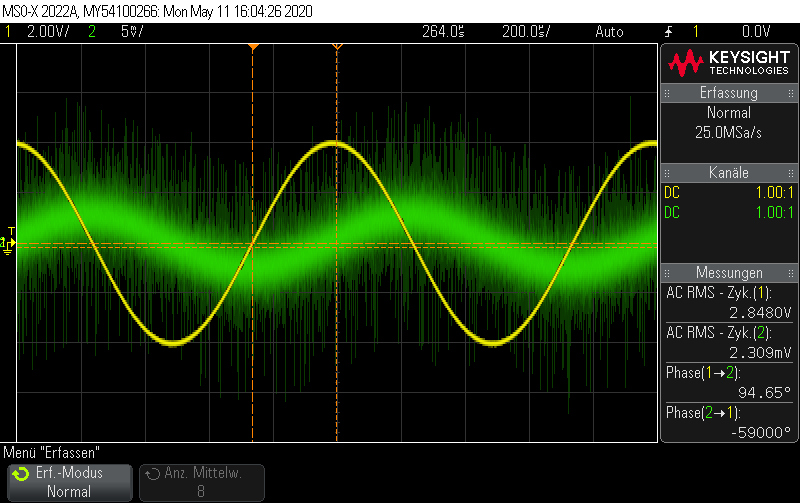
\includegraphics[width=\textwidth]{VERA/5_4/scope_5}
  \end{center}
  \caption{Verrauschtes Ausgangssignals (grün) am Oszilloskop}
  \label{fig:rauschi}
\end{figure}

\begin{figure}[H]
  \begin{center}
    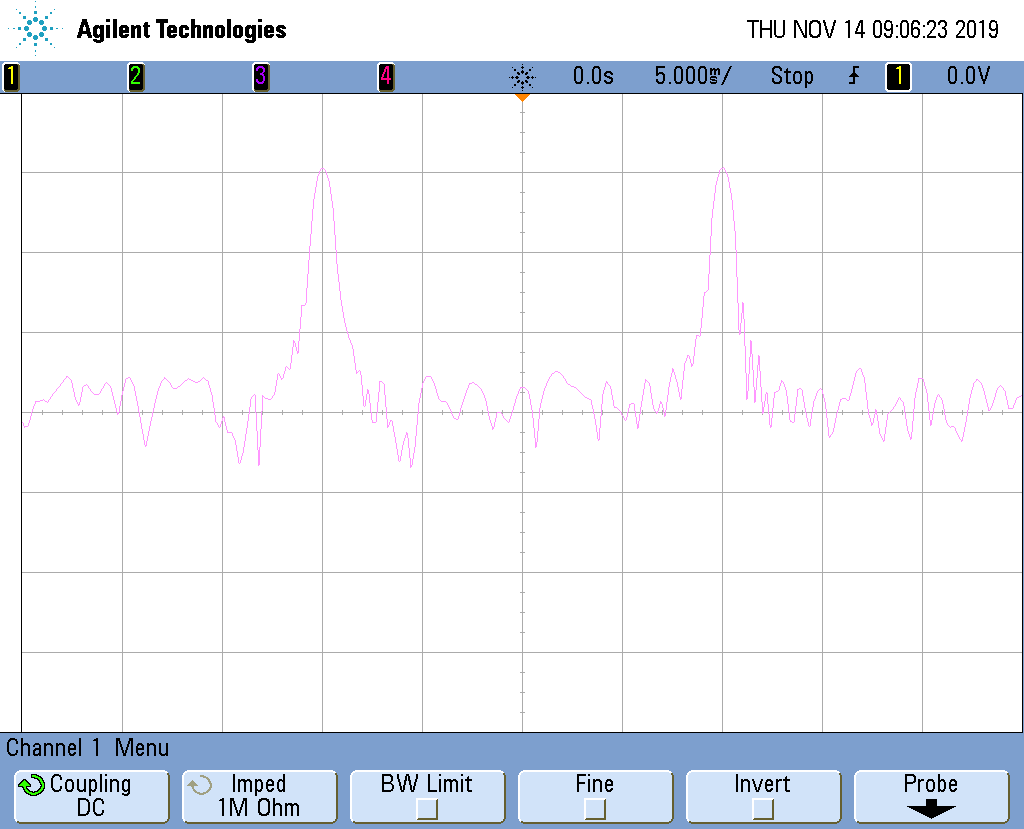
\includegraphics[width=\textwidth]{VERA/5_4/scope_6}
  \end{center}
  \caption{Rauschfreie Darstellung des Ausgangssignals}
\end{figure}

Die Messwerte sind
\[U_{\mathrm{a, f=1kHz}} = 1.84 \, \si{\milli\volt}_{\mathrm{RMS}}\]
\[U_{\mathrm{a, f=10kHz}} = 17.89 \, \si{\milli\volt}_{\mathrm{RMS}} \]

Daraus ergeben sich über
\[V_{GlT} = \frac{U_{\mathrm{a, eff}}}{U_{\mathrm{e, eff}}}\]

die Gleichtaktverstärkungen
\[V_{GlT, \mathrm{f=1kHz}} = 0.6505 = -3.7 \, \si{\deci\bel}\]
\[V_{GlT, \mathrm{f=10kHz}} = 6.3251 = 16 \, \si{\deci\bel}\]

bzw. invers als CMRR
\[\mathrm{CMMR}_{\mathrm{f=1kHz}} = 3.7 \, \si{\deci\bel}\]
\[\mathrm{CMMR}_{\mathrm{f=10kHz}} = -16 \, \si{\deci\bel}\]

\subsubsection{Gegentaktverstärkung}
Die Ausgangssignale wurden bei erdfreier Verbindung des Eingangssignals
mit $U_{e, \mathrm{pp}} = 1 \, \si{\volt}_{\mathrm{pp}}$ gemessen.
\[U_{\mathrm{a,f=1kHz}} = 4.967 \, \si{\volt}_{\mathrm{pp}}\]
\[U_{\mathrm{a,f=10kHz}} = 4.998 \, \si{\volt}_{\mathrm{pp}}\]

Die Gegentaktverstärkung ist somit
\[V_{GgT} = \frac{U_{a, pp}}{U_{e, pp}}\]
\[V_{GgT, \mathrm{f=1kHz}} = 4.967\]
\[V_{GgT, \mathrm{f=10kHz}} = 4.998\]
was dem eingestellten Verstärkungswert von $5$ entspricht.

\subsubsection{Mischspannungen}
Die Schaltung wurde dann mit verschiedenen Mischspannungen getestet. Am
invertierenden Eingang lag eine Gleichspannung, am nichtinvertierenden eine
Wechselspannung der Frequenz $f = 1\,\si{\kilo\hertz}$. Die Ergebnisse sind in Tabelle \ref{tab:misch} zu sehen.

% Please add the following required packages to your document preamble:
% \usepackage{booktabs}
% \usepackage[table,xcdraw]{xcolor}
% If you use beamer only pass "xcolor=table" option, i.e. \documentclass[xcolor=table]{beamer}
\begin{table}[H]
\begin{tabular}{@{}l|l|l|l@{}}
\rowcolor{gray1} 
$u_1$                         & $1 \si{\volt} \sin{\omega t}$                             & $1 \si{\volt} \sin{\omega t}$                                & $1 \si{\volt} \sin{\omega t}$                               \\
\rowcolor{gray1} 
$U_2$                         & $-0.5 \, \si{\volt}$                                    & $0 \, \si{\volt}$                                          & $0.5 \, \si{\volt}$                                       \\
\cellcolor{gray1}$u_a$ & $2.442 \, \si{\volt} + 4.97\,\si{\volt} \sin{\omega t}$ & $52 \, \si{\milli\volt} + 4.98\,\si{\volt} \sin{\omega t}$ & $-2.527 \, \si{\volt} - 4.975\,\si{\volt} \sin{\omega t}$
\end{tabular}
\caption{Messergebnisse bei Mischspannung}
\label{tab:misch}
\end{table}

Die Gleichspannungs- und Wechselspannungsanteile wurden wie erwartet
separat/distributiv mit der Verstärkung von $V=5$ verstärkt.